\documentclass[lang=cn,11pt,a4paper,cite=authornum]{paper}

\title{计算机网络课程设计:“DNS中继服务器”的实现\ 实验报告}
\author{毛子恒 \\ 2019211397 \and 李臻 \\ 2019211458 \and 张梓靖 \\ 2019211379}
\institute{北京邮电大学\ 计算机学院}

\date{\zhtoday}

% 本文档命令
\usepackage{array}
\newcommand{\ccr}[1]{\makecell{{\color{#1}\rule{1cm}{1cm}}}}
\nocite{*}

\begin{document}

\maketitle

\section{概览}

\subsection{任务描述}

\label{basic}设计一个DNS服务器程序,读入“IP地址-域名”对照表,当客户端查询域名对应的IP地址时,用域名检索该对照表:

\begin{itemize}
    \item 检索到IP地址0.0.0.0,则向客户端返回“域名不存在”的报错消息(不良网站拦截功能)
    \item 检索到普通IP地址,则向客户端返回该地址(服务器功能)
    \item 表中未检到该域名,则向因特网DNS服务器发出查询,并将结果返给客户端(中继功能)
\end{itemize}

\subsection{实验环境}

\begin{itemize}
    \item macOS Big Sur 11.3
    \item Apple clang version 12.0.5
    \item cmake version 3.19.1
    \item Clion 2021.1.1
    \item Visual Studio Code 1.56.2
\end{itemize}

\subsection{成员分工}

\section{功能需求}

\paragraph{基本需求}

细化\ref{basic}节指定的三个功能,我们提出如下几个基本需求:

\begin{enumerate}
    \item 解析和构建DNS报文。
    \item 监听本地53端口,获取DNS请求;将查询到的DNS回复发送回本地。
    \item 加载本地的“IP地址-域名”对照表,维护一个数据结构,用于增添、查询DNS记录。
    \item 将DNS请求发送到远程服务器的53端口,并且监听来自远程服务器的回复。
\end{enumerate}

\paragraph{额外需求}

此外,基于性能和实用性的考虑,我们实现了数个额外需求:

\begin{enumerate}
    \item 输出调试信息和DNS报文内容。
    \item 在转发DNS请求时重新分配序号,以区分不同的查询。
    \item 避免阻塞式查询,采用事件驱动的方式实现高并发。
    \item 对于数据结构中查询不到的DNS请求,存储来自服务器的DNS回复以供之后的重复查询,并且在到期后删除记录。
    \item 实现高速缓存,对于经常访问的记录,加快查询效率。
    \item 命令行参数解析。
\end{enumerate}

\section{模块介绍}

\subsection{DNS报文解析和构建}

\subsubsection{DNS报文格式分析}

一个DNS报文由如下五个部分构成:

\begin{code}
\begin{minted}[frame=none]{text}
+---------------------+
|        Header       |
+---------------------+
|       Question      |
+---------------------+
|        Answer       |
+---------------------+
|      Authority      |
+---------------------+
|      Additional     |
+---------------------+
\end{minted}
\end{code}

\paragraph{Header部分格式}

Header部分为报文头,Question部分的内容为向域名服务器的查询;之后的三个部分有相同的格式,即Resource Record(RR),并且都可能为空;Answer部分是对于查询的回复,Authority部分的内容指向权威域名服务器,Additional部分包含一些相关额外信息。

Header部分的结构如下:

\begin{code}
\begin{minted}[frame=none]{text}
  0  1  2  3  4  5  6  7  8  9 10 11 12 13 14 15
+--+--+--+--+--+--+--+--+--+--+--+--+--+--+--+--+
|                      ID                       |
+--+--+--+--+--+--+--+--+--+--+--+--+--+--+--+--+
|QR|   Opcode  |AA|TC|RD|RA|   Z    |   RCODE   |
+--+--+--+--+--+--+--+--+--+--+--+--+--+--+--+--+
|                    QDCOUNT                    |
+--+--+--+--+--+--+--+--+--+--+--+--+--+--+--+--+
|                    ANCOUNT                    |
+--+--+--+--+--+--+--+--+--+--+--+--+--+--+--+--+
|                    NSCOUNT                    |
+--+--+--+--+--+--+--+--+--+--+--+--+--+--+--+--+
|                    ARCOUNT                    |
+--+--+--+--+--+--+--+--+--+--+--+--+--+--+--+--+
\end{minted}
\end{code}

\begin{itemize}
    \item ID,用于由产生DNS查询的程序分配,用于标识一个请求;一对DNS查询和回复的ID相同。
    \item QR,查询报文此位为0,回复报文此位为1。
    \item OPCODE,查询的类型:
        \begin{itemize}
            \item 0,标准查询;
            \item 1,反向查询;
            \item 2,服务器状态请求。
        \end{itemize}
    \item AA,在回复报文中有效,如果为1,表示回复Question部分查询的域名服务器是权威服务器。
    \item TC,如果为1,说明这条消息由于信道的限制而被截断。
    \item RD,在查询报文中设置,如果为1,表示期望域名服务器递归查询这个请求。
    \item RA,在回复报文中设置,如果为1,表示递归查询在域名服务器中有效。
    \item Z,预留字段,全0.
    \item RCODE,回复状态编号:
        \begin{itemize}
            \item 0,没有错误;
            \item 1,查询格式错误;
            \item 2,由于服务器错误而无法处理查询;
            \item 3,域名错误,仅在权威服务器的回复中有意义,指查询中请求的域名不存在;
            \item 4,查询的类型不受支持;
            \item 5,服务器拒绝处理请求。
        \end{itemize}
    \item QDCOUNT,Question部分中查询记录的个数(通常是1)。
    \item ANCOUNT,Answer部分中RR的个数。
    \item NSCOUNT,Authority部分中RR的个数。
    \item ARCOUNT,Additional部分中RR的个数。
\end{itemize}

\paragraph{Question部分格式}

Question部分的结构如下:

\begin{code}
\begin{minted}[frame=none]{text}
  0  1  2  3  4  5  6  7  8  9 10 11 12 13 14 15
+--+--+--+--+--+--+--+--+--+--+--+--+--+--+--+--+
|                                               |
/                     QNAME                     /
/                                               /
+--+--+--+--+--+--+--+--+--+--+--+--+--+--+--+--+
|                     QTYPE                     |
+--+--+--+--+--+--+--+--+--+--+--+--+--+--+--+--+
|                     QCLASS                    |
+--+--+--+--+--+--+--+--+--+--+--+--+--+--+--+--+
\end{minted}
\end{code}

\begin{itemize}
    \item QNAME,查询域名,格式在\ref{name_format}节说明。
    \item QTYPE,查询类型,受支持的类型如下:
        \begin{itemize}
            \item 1,A,主机地址;
            \item 2,NS,权威域名服务器;
            \item 5,CNAME,域名引用;
            \item 6,SOA,授权机构起始;
            \item 12,PTR,域名指针,用于反向域名查找;
            \item 13,HINFO,主机信息;
            \item 14,MINFO,邮箱或邮件列表信息;
            \item 15,MX,邮件交换;
            \item 16,TXT,字符串。
            \item 28,AAAA,IPv6地址。
        \end{itemize}
    \item QCLASS,查询类别,仅支持1,IN,因特网。
\end{itemize}

\paragraph{Resource Record格式}

Resource Record的格式如下:

\begin{code}
\begin{minted}[frame=none]{text}
  0  1  2  3  4  5  6  7  8  9 10 11 12 13 14 15
+--+--+--+--+--+--+--+--+--+--+--+--+--+--+--+--+
|                                               |
/                      NAME                     /
/                                               /
+--+--+--+--+--+--+--+--+--+--+--+--+--+--+--+--+
|                      TYPE                     |
+--+--+--+--+--+--+--+--+--+--+--+--+--+--+--+--+
|                     CLASS                     |
+--+--+--+--+--+--+--+--+--+--+--+--+--+--+--+--+
|                      TTL                      |
|                                               |
+--+--+--+--+--+--+--+--+--+--+--+--+--+--+--+--+
|                    RDLENGTH                   |
+--+--+--+--+--+--+--+--+--+--+--+--+--+--+--+--+
|                                               |
/                     RDATA                     /
/                                               /
+--+--+--+--+--+--+--+--+--+--+--+--+--+--+--+--+
\end{minted}
\end{code}

\begin{itemize}
    \item NAME,此RR从属的域名,格式在\ref{name_format}节说明。
    \item TYPE,RR类型,支持的类型与QTYPE部分相同。
    \item CLASS,RR类别,仅支持1,IN,因特网。
    \item TTL,期望此RR被缓存的时间。
    \item RDLENGTH,RDATA部分的长度。
    \item RDATA,资源内容,根据TYPE的不同,其内容也不同。
\end{itemize}

\paragraph{域名格式}
\label{name_format}

Question部分和RR中的域名都是由一串字符\mintinline{text}{<domain-name>}表示,一般由0表示终止,其长度任意,并且不包含填充。
\mintinline{text}{<domain-name>}由若干个\mintinline{text}{<character-string>}构成,每个\mintinline{text}{<character-string>}由一个八位数字开头,之后跟着长度等于这个数字的字符串。\mintinline{text}{<character-string>}最多包含256个字符。

为了压缩DNS报文的长度,增大传输效率,引入了域名的压缩,此时\mintinline{text}{<domain-name>}可能由0或者一个指针终止,一个指针由两个字节构成,其格式如下:

\begin{code}
\begin{minted}[frame=none]{text}
+--+--+--+--+--+--+--+--+--+--+--+--+--+--+--+--+
| 1  1|                OFFSET                   |
+--+--+--+--+--+--+--+--+--+--+--+--+--+--+--+--+
\end{minted}
\end{code}

这个指针指向从DNS报文头起第\mintinline{text}{OFFSET}个字节,原本域名的剩余部分应该从这个字节开始继续读取。

\paragraph{RDATA格式}

对于DNS中继服务器来说,RDATA部分的内容并不重要,只是涉及到域名压缩,以及调试输出的需求,所以需要对一部分类型的RDATA作处理。需要处理的RDATA如下。

\subparagraph{A类型RDATA格式}

如下:

\begin{code}
\begin{minted}[frame=none]{text}
    +--+--+--+--+--+--+--+--+--+--+--+--+--+--+--+--+
    |                    ADDRESS                    |
    +--+--+--+--+--+--+--+--+--+--+--+--+--+--+--+--+
\end{minted}
\end{code}

\begin{itemize}
    \item ADDRESS,32位IPv4地址。
\end{itemize}

\subparagraph{NS/CNAME类型RDATA格式}

如下:

\begin{code}
\begin{minted}[frame=none]{text}
    +--+--+--+--+--+--+--+--+--+--+--+--+--+--+--+--+
    |                     NAME                      |
    +--+--+--+--+--+--+--+--+--+--+--+--+--+--+--+--+
\end{minted}
\end{code}

\begin{itemize}
    \item NAME,一个域名。
\end{itemize}

\subparagraph{MX类型RDATA格式}

如下:

\begin{code}
\begin{minted}[frame=none]{text}
    +--+--+--+--+--+--+--+--+--+--+--+--+--+--+--+--+
    |                  PREFERENCE                   |
    +--+--+--+--+--+--+--+--+--+--+--+--+--+--+--+--+
    |                   EXCHANGE                    |
    +--+--+--+--+--+--+--+--+--+--+--+--+--+--+--+--+
\end{minted}
\end{code}

\begin{itemize}
    \item PREFERENCE,16位数字。
    \item EXCHANGE,一个域名。
\end{itemize}

\subparagraph{SOA类型RDATA格式}

如下:

\begin{code}
\begin{minted}[frame=none]{text}
    +--+--+--+--+--+--+--+--+--+--+--+--+--+--+--+--+
    |                                               |
    /                     MNAME                     /
    /                                               /
    +--+--+--+--+--+--+--+--+--+--+--+--+--+--+--+--+
    |                                               |
    /                     RNAME                     /
    /                                               /
    +--+--+--+--+--+--+--+--+--+--+--+--+--+--+--+--+
    |                    SERIAL                     |
    |                                               |
    +--+--+--+--+--+--+--+--+--+--+--+--+--+--+--+--+
    |                    REFRESH                    |
    |                                               |
    +--+--+--+--+--+--+--+--+--+--+--+--+--+--+--+--+
    |                     RETRY                     |
    |                                               |
    +--+--+--+--+--+--+--+--+--+--+--+--+--+--+--+--+
    |                    EXPIRE                     |
    |                                               |
    +--+--+--+--+--+--+--+--+--+--+--+--+--+--+--+--+
    |                    MINIMUM                    |
    |                                               |
    +--+--+--+--+--+--+--+--+--+--+--+--+--+--+--+--+
\end{minted}
\end{code}

\begin{itemize}
    \item MNAME,一个域名。
    \item RNAME,一个域名。
    \item SERIAL,一个32位数字。
    \item REFRESH,一个32位数字。
    \item RETRY,一个32位数字。
    \item EXPIRE,一个32位数字。
    \item MINIMUM,一个32位数字。
\end{itemize}

\subparagraph{AAAA类型RDATA格式}

如下:

\begin{code}
\begin{minted}[frame=none]{text}
    +--+--+--+--+--+--+--+--+--+--+--+--+--+--+--+--+
    |                                               |
    |                                               |
    |                                               |
    |                    ADDRESS                    |
    |                                               |
    |                                               |
    |                                               |
    |                                               |
    +--+--+--+--+--+--+--+--+--+--+--+--+--+--+--+--+
\end{minted}
\end{code}

\begin{itemize}
    \item ADDRESS,128位IPv6地址。
\end{itemize}

\subsubsection{DNS报文结构体}

DNS报文结构体定义在\mintinline{text}{dns_structure.h}中,由四个结构体构成,其结构如\figref{fig:struct_structure}所示。

\begin{figure}[htbp]

    \centering
    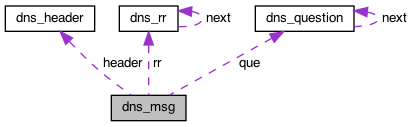
\includegraphics[width=0.7\linewidth]{./APIdoc/structdns__msg__coll__graph.png}
    \caption{DNS报文结构体的结构\label{fig:struct_structure}}

\end{figure}

Header部分长度固定,其中部分不足一个字节的字段采用位域(bit field)的方式定义,节省空间;
Question部分的查询记录个数不定,采用单向链表实现,便于顺序访问;之后的Answer、Authority和Additional部分的格式相同,采用一个单向链表顺序连接起来。

四个结构体的定义如下所示:

\begin{code}
\begin{minted}{C}
typedef struct dns_header
{
    uint16_t id;
    uint8_t qr: 1;
    uint8_t opcode: 4;
    uint8_t aa: 1;
    uint8_t tc: 1;
    uint8_t rd: 1;
    uint8_t ra: 1;
    uint8_t z: 3;
    uint8_t rcode: 4;
    uint16_t qdcount;
    uint16_t ancount;
    uint16_t nscount;
    uint16_t arcount;
} Dns_Header;
 
typedef struct dns_question
{
    uint8_t * qname;
    uint16_t qtype;
    uint16_t qclass;
    struct dns_question * next;
} Dns_Que;
 
typedef struct dns_rr
{
    uint8_t * name;
    uint16_t type;
    uint16_t class;
    uint32_t ttl;
    uint16_t rdlength;
    uint8_t * rdata;
    struct dns_rr * next;
} Dns_RR;
 
typedef struct dns_msg
{
    Dns_Header * header; 
    Dns_Que * que; 
    Dns_RR * rr; 
} Dns_Msg;
\end{minted}
\end{code}

\mintinline{text}{dns_structure.h}的文档见\href{run:./APIdoc/dns__structure_8h.html}{dns\_structure.h文件参考}。

\subsubsection{DNS报文字节流和结构体的转换}

从UDP socket中获取到的DNS报文是字节流的形式,我们需要将它转换成结构体,便于分析与输出,之后需要将结构体转换回字节流进行发送。

此外,我们还需要关注报文结构体和RR结构体的复制和销毁操作。

上述操作定义在\mintinline{text}{dns_conversion.h}中,如下:

\begin{code}
\begin{minted}{C}
void string_to_dnsmsg(Dns_Msg * pmsg, const char * pstring);

unsigned dnsmsg_to_string(const Dns_Msg * pmsg, char * pstring);
 
void destroy_dnsrr(Dns_RR * prr);
 
void destroy_dnsmsg(Dns_Msg * pmsg);
 
Dns_RR * copy_dnsrr(const Dns_RR * src);
 
Dns_Msg * copy_dnsmsg(const Dns_Msg * src);
\end{minted}
\end{code}

\mintinline{text}{dns_conversion.h}的文档见\href{run:./APIdoc/dns__conversion_8h.html}{dns\_conversion.h文件参考}。

\paragraph{将字节流转换成结构体}

\mintinline{C}{string_to_dnsmsg}函数实现将字节流转换成结构体,它的函数调用图如\figref{fig:string_to_dnsmsg_call}。

\begin{figure}[htbp]

    \centering
    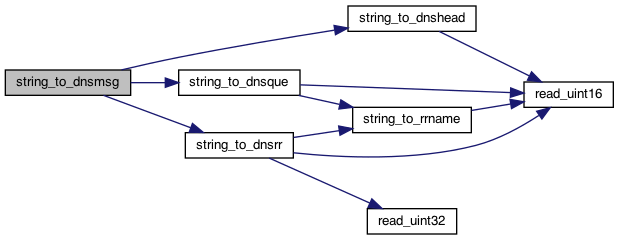
\includegraphics[width=0.7\linewidth]{./APIdoc/dns__conversion_8c_a0f89102e256c499ffa19784791cb68f6_cgraph.png}
    \caption{\mintinline{C}{string_to_dnsmsg}函数调用图\label{fig:string_to_dnsmsg_call}}

\end{figure}

从图中可见,此函数分别调用\mintinline{C}{string_to_dnshead}、\mintinline{C}{string_to_dnsque}和\mintinline{C}{string_to_dnsrr}将报文的三个部分转换为结构体,对于Question部分和RR部分,需要维护一个链表头指针和尾指针,每次转换后的新记录插入链表尾即可。

此外,考虑到域名格式的特殊性,\mintinline{C}{string_to_rrname}函数负责通过递归的形式将域名解析成可输出的常见的格式,\mintinline{C}{read_uint16}和\mintinline{C}{read_uint32}函数用于将大端法数字转换成小端法数字。

\paragraph{将结构体转换成字节流}

\mintinline{C}{dnsmsg_to_string}函数实现将结构体转换成字节流,它的函数调用图如\figref{fig:dnsmsg_to_string_call}。

\begin{figure}[htbp]

    \centering
    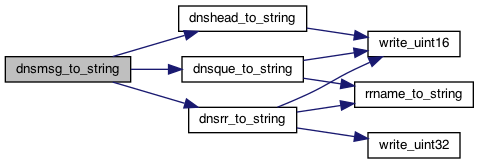
\includegraphics[width=0.7\linewidth]{./APIdoc/dns__conversion_8c_aa893e182a92c2ccf5644c1f8a12fba37_cgraph.png}
    \caption{\mintinline{C}{dnsmsg_to_string}函数调用图\label{fig:dnsmsg_to_string_call}}

\end{figure}

\mintinline{C}{dnsmsg_to_string}函数基本上是\mintinline{C}{string_to_dnsmsg}的逆过程,分别调用类似的六个函数实现相应的功能。

\paragraph{结构体的销毁}

\mintinline{C}{destroy_dnsmsg}和\mintinline{C}{destroy_dnsrr}函数分别实现整个DNS报文的销毁和RR链表的销毁。

\paragraph{结构体的复制}

\mintinline{C}{copy_dnsmsg}和\mintinline{C}{copy_dnsrr}函数分别实现整个DNS报文的复制和RR链表的复制。

上面提到的函数接口的的文档见\href{run:./APIdoc/dns__conversion_8c.html}{dns\_conversion.c文件参考}。

\subsubsection{DNS报文的输出}

通过输出DNS字节流和结构体,可以观察DNS报文的转换过程是否正确,并且跟踪程序运行的过程,便于debug的工作。

上述操作定义在\mintinline{text}{dns_print.h}中,如下:

\begin{code}
\begin{minted}{C}
void print_dns_string(const char * pstring, unsigned int len);
 
void print_dns_message(const Dns_Msg * pmsg);
\end{minted}
\end{code}

\mintinline{text}{dns_print.h}的文档见\href{run:./APIdoc/dns__print_8h.html}{dns\_print.h文件参考}。

\mintinline{C}{print_dns_string}函数用于输出DNS字节流,输出的效果如下:

\begin{code}
\begin{minted}[frame=none]{text}
0000 bd da 81 80 00 01 00 01 00 00 00 00 03 77 77 77 
0010 04 62 75 70 74 03 65 64 75 02 63 6e 00 00 01 00 
0020 01 03 77 77 77 04 62 75 70 74 03 65 64 75 02 63 
0030 6e 00 00 01 00 01 ff ff ff ff 00 04 0a 03 09 a1 
\end{minted}
\end{code}

\mintinline{C}{print_dns_message}函数用于输出DNS结构体,其函数调用图如\figref{fig:print_dns_message_call}。

\begin{figure}[htbp]

    \centering
    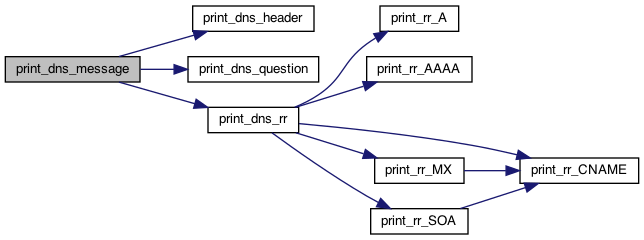
\includegraphics[width=0.7\linewidth]{./APIdoc/dns__print_8c_a33a39397e0f2e1a98b86b6d85321ee79_cgraph.png}
    \caption{\mintinline{C}{print_dns_message}函数调用图\label{fig:print_dns_message_call}}

\end{figure}

该函数分别调用\mintinline{C}{print_dns_header}、\mintinline{C}{print_dns_question}和\mintinline{C}{print_dns_rr}函数输出结构体的三个部分。
由于RR的RDATA字段格式较多,所以另外实现了几个函数用于输出不同类型的RDATA字段。

输出的效果如下:

\begin{code}
\begin{minted}[frame=none]{text}
=======Header==========
ID = 0xbdda
QR = 1
OPCODE = 0
AA = 0
TC = 0
RD = 1
RA = 1
RCODE = 0
QDCOUNT = 1
ANCOUNT = 1
NSCOUNT = 0
ARCOUNT = 0

=======Question========
QNAME = www.bupt.edu.cn.
QTYPE = 1
QCLASS = 1

=======Answer==========
NAME = www.bupt.edu.cn.
TYPE = 1
CLASS = 1
TTL = 4294967295
RDLENGTH = 4
RDATA = 10.3.9.161

=======Authority=======
=======Additional======
\end{minted}
\end{code}

上面提到的函数接口的的文档见\href{run:./APIdoc/dns__print_8c.html}{dns\_print.c文件参考}。

\subsection{DNS记录的存储}

理论上,通过一个域名和类型可以查询到一个RR的列表作为回复。对于DNS记录的存储就是基于这个对应关系。

\subsubsection{红黑树和RR链表}

DNS记录存储在一个红黑树中,红黑树节点的键是域名字符串经过哈希得到的整数,由于哈希可能存在冲突,并且一个域名可能对应多个不同类的查询,可采用拉链法解决冲突。
因此,每个红黑树节点对应多个值,这些值被串联成一个有空头结点的单向链表。每个值中存储域名和查询类型、一个RR的列表和RR列表中各个部分的个数。

上述数据结构的结构体的关系如\figref{fig:rbtree_structure}所示。

\begin{figure}[htbp]

    \centering
    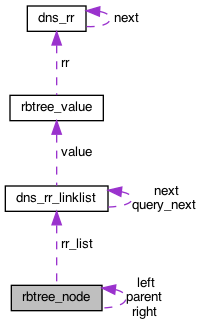
\includegraphics[width=0.3\linewidth]{./APIdoc/structrbtree__node__coll__graph.png}
    \caption{红黑树和RR链表结构体的关系\label{fig:rbtree_structure}}

\end{figure}

红黑树中会存储从对照表中读取到的”IP地址-域名“对,也会存储运行时收到的回复。当存储对照表中的记录时,默认这些记录是永久的,而存储运行时的回复时,需要根据RR列表中最小的TTL确认这条记录的过期时间,过期时间记录在链表的节点中。

此外,红黑树和RR链表(以及之后的大部分数据结构)都将数据结构的操作作为函数指针封装在结构体中,达到类似成员函数的效果。

红黑树和RR链表的数据结构和操作定义在\mintinline{text}{rbtree.h}中,如下:

\begin{code}
\begin{minted}{C}
typedef enum
{
    BLACK, RED
} Color;
 
typedef struct rbtree_value
{
    Dns_RR * rr; 
    uint16_t ancount; 
    uint16_t nscount; 
    uint16_t arcount; 
    uint8_t type; 
} Rbtree_Value;
 
typedef struct dns_rr_linklist
{
    Rbtree_Value * value; 
    time_t expire_time; 
    struct dns_rr_linklist * next; 
    
    void (* insert)(struct dns_rr_linklist * list, struct dns_rr_linklist * new_list_node);
    
    void (* delete_next)(struct dns_rr_linklist * list);
    
    struct dns_rr_linklist * (* query_next)(struct dns_rr_linklist * list, const uint8_t * qname, const uint16_t qtype);
} Dns_RR_LinkList;
 
typedef struct rbtree_node
{
    unsigned int key; 
    Dns_RR_LinkList * rr_list; 
    Color color; 
    struct rbtree_node * left; 
    struct rbtree_node * right; 
    struct rbtree_node * parent; 
} Rbtree_Node;
 
typedef struct rbtree
{
    Rbtree_Node * root; 
    
    void (* insert)(struct rbtree * tree, unsigned int key, Dns_RR_LinkList * list);
    
    Dns_RR_LinkList * (* query)(struct rbtree * tree, unsigned int data);
} Rbtree;
 
Dns_RR_LinkList * new_linklist();
 
Rbtree * new_rbtree();
\end{minted}
\end{code}

\mintinline{text}{rbtree.h}的文档见\href{run:./APIdoc/rbtree_8h.html}{rbtree.h文件参考}。

\paragraph{RR链表}

\mintinline{C}{Dns_RR_LinkList}结构体有三个方法:

\begin{itemize}
    \item \mintinline{C}{insert}方法用于在链表中的某个节点后插入新节点。
    \item \mintinline{C}{delete_next}方法用于删除链表中某个节点的下一个结点。
    \item \mintinline{C}{query_next}方法用于遍历一个链表,根据域名和查询类型从中筛选出一个节点。
\end{itemize}

\paragraph{红黑树的插入操作}

\mintinline{C}{Rbtree}结构体的\mintinline{C}{insert}方法用于向红黑树中插入键-值对。

具体来说,函数传入一个键和一个RR链表节点。首先在红黑树中按照键查找对应的节点,如果查找到节点,则将RR链表节点插入这个节点的RR链表尾;如果查找不到节点,则创建一个新节点以及一个有空头结点的RR链表,并将传入的RR链表节点插入到这个链表尾,在此之后,需要调用\mintinline{C}{insert_case}函数维护红黑树的平衡。

对于红黑树的维护细节不属于本报告的范畴,故略去。

这个方法对应\mintinline{text}{rbtree.c}中的\mintinline{C}{rbtree_insert}函数,该函数的调用图如\figref{fig:rbtree_insert_call}所示。

\begin{figure}[htbp]

    \centering
    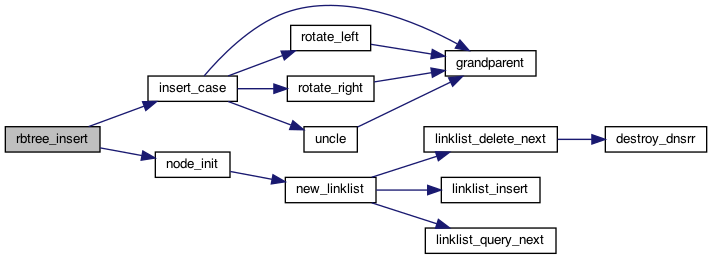
\includegraphics[width=0.8\linewidth]{./APIdoc/rbtree_8c_ae46c23eec5c1ea21ebab9279843de3a3_cgraph.png}
    \caption{\mintinline{C}{rbtree_insert}函数的调用图\label{fig:rbtree_insert_call}}

\end{figure}

\paragraph{红黑树的查询操作}

\mintinline{C}{Rbtree}结构体的\mintinline{C}{query}方法用于根据键在红黑树中查询RR链表。

函数调用\mintinline{C}{rbtree_find}函数,在红黑树中根据键查找结点。如果查找到节点,将节点的RR链表中超时的节点删去。如果此时节点的链表为空(即只有一个头节点),则调用\mintinline{C}{rbtree_delete}函数删除这个节点,并且维护红黑树的平衡;否则返回这个RR链表。

这个方法对应\mintinline{text}{rbtree.c}中的\mintinline{C}{rbtree_query}函数,该函数的调用图如\figref{fig:rbtree_query_call}所示。

\begin{figure}[htbp]

    \centering
    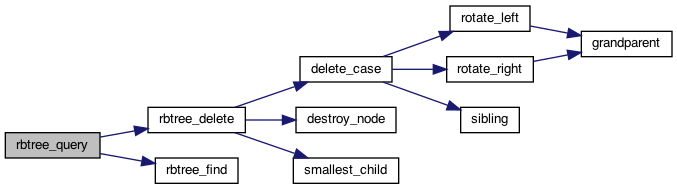
\includegraphics[width=0.8\linewidth]{./APIdoc/rbtree_8c_a7460cf092b0132ece0a692cd84a26456_cgraph.png}
    \caption{\mintinline{C}{rbtree_query}函数的调用图\label{fig:rbtree_query_call}}

\end{figure}

上面提到的函数接口的的文档见\href{run:./APIdoc/rbtree_8c.html}{rbtree.c文件参考}。

\subsubsection{LRU高速缓存}

\paragraph{缓存的插入操作}

\paragraph{缓存的查询操作}

\subsection{序号池和查询池}

\subsubsection{队列}

\subsubsection{序号池}

\subsubsection{查询池}

\subsection{DNS服务端和客户端}

\subsubsection{DNS服务端}

\subsubsection{DNS客户端}

\subsection{其他工具模块}

\subsubsection{命令行参数解析}

\subsubsection{调试信息输出}

\section{构建方式}

\section{测试结果}

\section{实验总结}

% \begin{figure}[htbp]

%     \centering
    
%     \subfigure[DHCP Discover]{
%         \begin{minipage}[t]{0.45\linewidth}
%             \centering
%             % \includegraphics[width=\linewidth]{./Images/DHCP1.png}
%         \end{minipage}
%     }
%     \subfigure[DHCP Offer]{
%         \begin{minipage}[t]{0.45\linewidth}
%             \centering
%             % \includegraphics[width=\linewidth]{./Images/DHCP2.png}
%         \end{minipage}
%     }
    
%     \subfigure[DHCP Request]{
%         \begin{minipage}[t]{0.45\linewidth}
%             \centering
%             % \includegraphics[width=\textwidth]{./Images/DHCP3-1.png}
%             % \includegraphics[width=\textwidth]{./Images/DHCP3-2.png}
%         \end{minipage}
%     }
%     \subfigure[DHCP ACK]{
%         \begin{minipage}[t]{0.45\linewidth}
%             \centering
%             % \includegraphics[width=\textwidth]{./Images/DHCP4-1.png}
%             % \includegraphics[width=\textwidth]{./Images/DHCP4-2.png}
%         \end{minipage}
%     }
%     \caption{四个DHCP分组的内容\label{fig:dhcp}}

% \end{figure}

% \begin{table}[!htbp]
%     \centering
%     \caption{DHCP Discover分组内容分析\label{tab:dhcp1res}}
%     \begin{tabular}{|c|c|l|}
%         \hline
%         字段 (字节数) & 内容(16进制) & 解释 \\
%         \hline
%         OP (1) & 01 & 消息类型:引导请求 \\
%         \hline
%         HTYPE (1) & 01 & 硬件地址类型:以太网 \\
%         \hline
%         HLEN (1) & 06 & 硬件地址长度:6 \\
%         \hline
%         HOPS (1) & 00 & 经过的DHCP中继的数目:0 \\
%         \hline
%         XID (4) & e8 75 52 dd & 处理ID,标记一次IP地址请求过程:0xe87552dd \\
%         \hline
%         SECS (2) & 00 00 & 从获取到IP地址或者续约过程开始到现在所消耗的时间:0秒 \\
%         \hline
%         FLAGS (2) & 00 00 & 标记:第一位为0,表示单播 \\
%         \hline
%         CIADDR (4) & 00 00 00 00 & \makecell[l]{客户端IP地址:0.0.0.0 \\ 还未分配IP地址} \\
%         \hline
%         YIADDR (4) & 00 00 00 00 & \makecell[l]{你的(客户端)IP地址(服务器分配的地址):0.0.0.0 \\ 仅在Offer和ACK分组中有效} \\
%         \hline
%         SIADDR (4) & 00 00 00 00 & \makecell[l]{在bootstrap过程中下一台服务器的地址:0.0.0.0 \\ DHCP服务器未知} \\
%         \hline
%         GIADDR (4) & 00 00 00 00 & \makecell[l]{客户端发出请求分组后经过的第一个中继的地址:0.0.0.0 \\ 没有经过中继} \\
%         \hline
%         CHADDR (16) & 58 a0 23 71 25 14 & \makecell[l]{客户端的MAC地址:58:a0:23:71:25:14 \\ 后接10个字节的填充} \\
%         \hline
%         SNAME (64) & 全部为00 & 为客户端分配IP地址的服务器域名:未给出 \\
%         \hline
%         FILE (128) & 全部为00 & 为启动客户端指定的配置文件路径:未给出 \\
%         \hline
%         \makecell[c]{magic \\ cookie(4)} & 63 82 53 63 & 可选字段的格式:DHCP \\
%         \hline
%         OPTION (3) & 35 01 01 & DHCP消息类型:Discover \\
%         \hline
%         OPTION (9) & \makecell[c]{3d 07 01 \\ 58 a0 23 71 25 14} & 客户端标识符:以太网,MAC地址58:a0:23:71:25:14 \\
%         \hline
%         OPTION (17) & 0c 0f 后略 & 主机名,长度为15 \\
%         \hline
%         OPTION (8) & 3c 08 后略 & 供应商标识符,长度为8 \\
%         \hline
%         OPTION (16) & 37 0e 后略 & 参数需求列表,长度为14 \\
%         \hline
%         OPTION (1) & ff & 选项字段结束 \\
%         \hline
%     \end{tabular}
% \end{table}

\end{document}